% Options for packages loaded elsewhere
\PassOptionsToPackage{unicode}{hyperref}
\PassOptionsToPackage{hyphens}{url}
%
\documentclass[
]{article}
\usepackage{amsmath,amssymb}
\usepackage{lmodern}
\usepackage{ifxetex,ifluatex}
\ifnum 0\ifxetex 1\fi\ifluatex 1\fi=0 % if pdftex
  \usepackage[T1]{fontenc}
  \usepackage[utf8]{inputenc}
  \usepackage{textcomp} % provide euro and other symbols
\else % if luatex or xetex
  \usepackage{unicode-math}
  \defaultfontfeatures{Scale=MatchLowercase}
  \defaultfontfeatures[\rmfamily]{Ligatures=TeX,Scale=1}
\fi
% Use upquote if available, for straight quotes in verbatim environments
\IfFileExists{upquote.sty}{\usepackage{upquote}}{}
\IfFileExists{microtype.sty}{% use microtype if available
  \usepackage[]{microtype}
  \UseMicrotypeSet[protrusion]{basicmath} % disable protrusion for tt fonts
}{}
\makeatletter
\@ifundefined{KOMAClassName}{% if non-KOMA class
  \IfFileExists{parskip.sty}{%
    \usepackage{parskip}
  }{% else
    \setlength{\parindent}{0pt}
    \setlength{\parskip}{6pt plus 2pt minus 1pt}}
}{% if KOMA class
  \KOMAoptions{parskip=half}}
\makeatother
\usepackage{xcolor}
\IfFileExists{xurl.sty}{\usepackage{xurl}}{} % add URL line breaks if available
\IfFileExists{bookmark.sty}{\usepackage{bookmark}}{\usepackage{hyperref}}
\hypersetup{
  pdftitle={SPAN Stage One Report},
  pdfauthor={Ryan P. Cabeen},
  hidelinks,
  pdfcreator={LaTeX via pandoc}}
\urlstyle{same} % disable monospaced font for URLs
\usepackage[margin=1in]{geometry}
\usepackage{graphicx}
\makeatletter
\def\maxwidth{\ifdim\Gin@nat@width>\linewidth\linewidth\else\Gin@nat@width\fi}
\def\maxheight{\ifdim\Gin@nat@height>\textheight\textheight\else\Gin@nat@height\fi}
\makeatother
% Scale images if necessary, so that they will not overflow the page
% margins by default, and it is still possible to overwrite the defaults
% using explicit options in \includegraphics[width, height, ...]{}
\setkeys{Gin}{width=\maxwidth,height=\maxheight,keepaspectratio}
% Set default figure placement to htbp
\makeatletter
\def\fps@figure{htbp}
\makeatother
\setlength{\emergencystretch}{3em} % prevent overfull lines
\providecommand{\tightlist}{%
  \setlength{\itemsep}{0pt}\setlength{\parskip}{0pt}}
\setcounter{secnumdepth}{-\maxdimen} % remove section numbering
\usepackage{booktabs}
\usepackage{makecell}
\ifluatex
  \usepackage{selnolig}  % disable illegal ligatures
\fi

\title{SPAN Stage One Report}
\author{Ryan P. Cabeen}
\date{2021-03-31}

\begin{document}
\maketitle

\newpage

\hypertarget{image-quality}{%
\section{Image quality}\label{image-quality}}

\begin{center}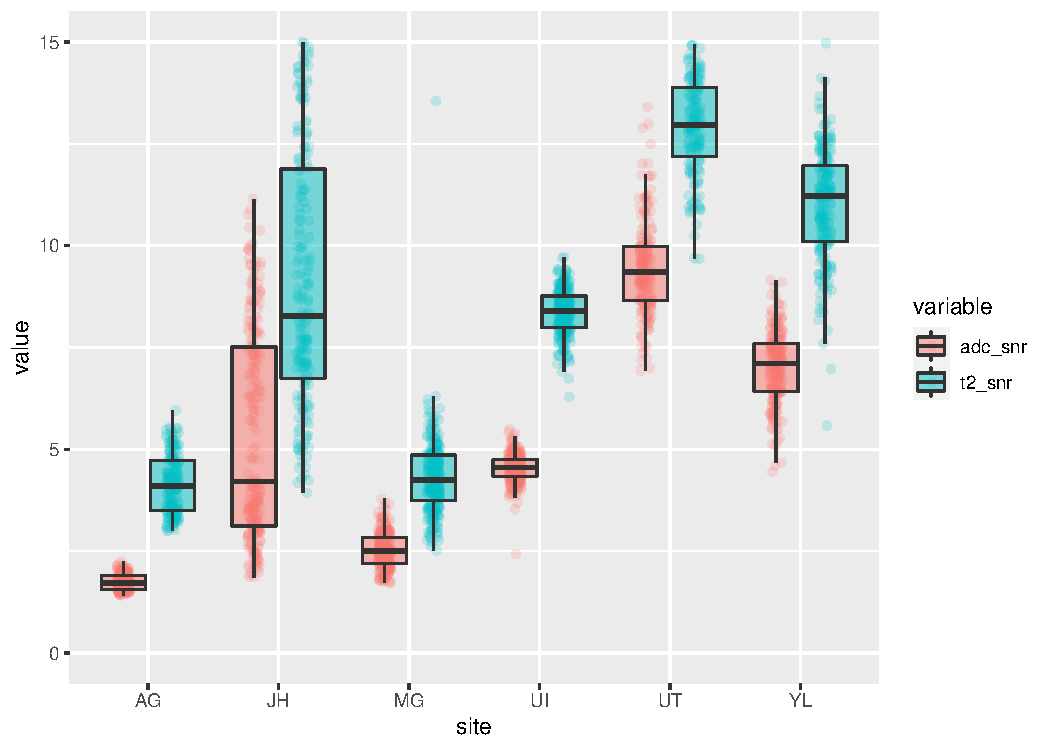
\includegraphics{paper_files/figure-latex/plot_snr-1} \end{center}

\begin{table}[ht]
\centering
\begin{tabular}{rllrrrrrr}
  \hline
 & site & variable & num & mean & sd & min & max & cv \\ 
  \hline
1 & AG & adc\_snr & 188 & 1.74 & 0.20 & 1.42 & 2.25 & 0.11 \\ 
  2 & AG & t2\_snr & 188 & 4.14 & 0.71 & 3.00 & 5.96 & 0.17 \\ 
  3 & JH & adc\_snr & 226 & 5.35 & 2.56 & 1.86 & 11.14 & 0.48 \\ 
  4 & JH & t2\_snr & 226 & 10.41 & 4.05 & 3.93 & 19.32 & 0.39 \\ 
  5 & MG & adc\_snr & 244 & 2.64 & 1.75 & 1.72 & 28.97 & 0.66 \\ 
  6 & MG & t2\_snr & 244 & 4.31 & 0.98 & 2.51 & 13.55 & 0.23 \\ 
  7 & UI & adc\_snr & 259 & 4.54 & 0.34 & 2.43 & 5.49 & 0.07 \\ 
  8 & UI & t2\_snr & 259 & 8.37 & 0.56 & 6.28 & 9.72 & 0.07 \\ 
  9 & UT & adc\_snr & 176 & 9.45 & 1.16 & 6.94 & 13.41 & 0.12 \\ 
  10 & UT & t2\_snr & 176 & 13.27 & 1.51 & 9.68 & 17.61 & 0.11 \\ 
  11 & YL & adc\_snr & 203 & 7.02 & 0.88 & 4.45 & 9.15 & 0.13 \\ 
  12 & YL & t2\_snr & 203 & 10.99 & 1.38 & 5.58 & 14.97 & 0.13 \\ 
   \hline
\end{tabular}
\end{table}
\begin{table}[ht]
\centering
\begin{tabular}{rlrrrrrr}
  \hline
 & variable & num & mean & sd & min & max & cv \\ 
  \hline
1 & adc\_snr & 1296 & 4.97 & 2.83 & 1.42 & 28.97 & 0.57 \\ 
  2 & t2\_snr & 1296 & 8.42 & 3.81 & 2.51 & 19.32 & 0.45 \\ 
   \hline
\end{tabular}
\end{table}

\hypertarget{total-brain-volume}{%
\section{Total brain volume}\label{total-brain-volume}}

\begin{center}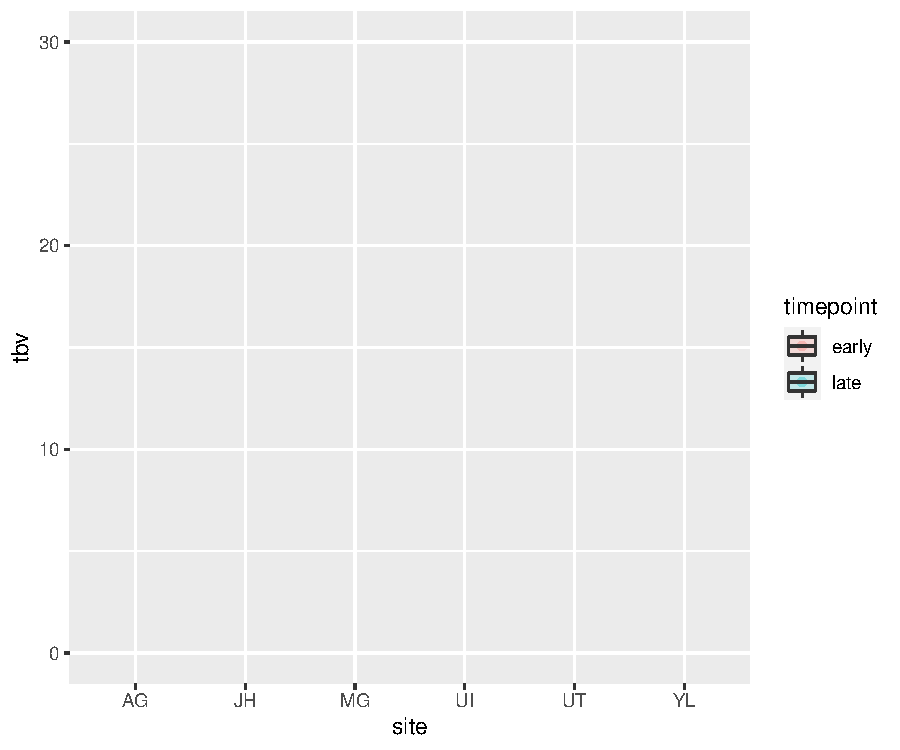
\includegraphics{paper_files/figure-latex/plot_tbv_site-1} \end{center}

\begin{center}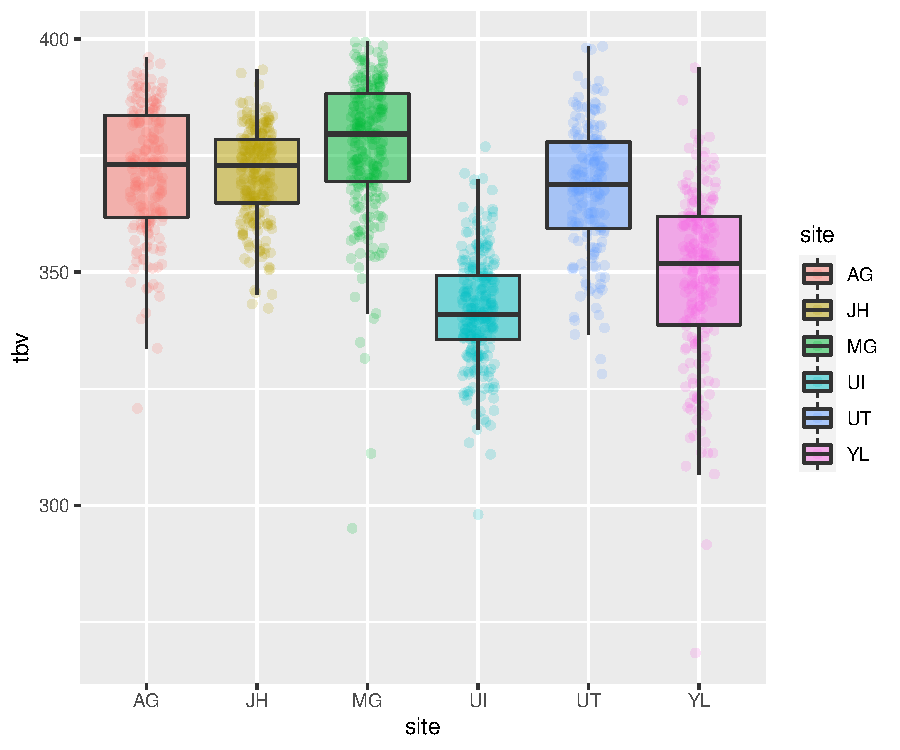
\includegraphics{paper_files/figure-latex/plot_tbv-1} \end{center}

\begin{table}[ht]
\centering
\begin{tabular}{rllrrrrrr}
  \hline
 & site & variable & num & mean & sd & min & max & cv \\ 
  \hline
1 & AG & tbv & 188 & 371.65 & 13.61 & 320.74 & 396.06 & 0.04 \\ 
  2 & JH & tbv & 226 & 370.99 & 9.93 & 342.23 & 393.40 & 0.03 \\ 
  3 & MG & tbv & 244 & 377.05 & 14.65 & 295.03 & 399.36 & 0.04 \\ 
  4 & UI & tbv & 259 & 341.79 & 11.63 & 298.01 & 376.89 & 0.03 \\ 
  5 & UT & tbv & 176 & 367.91 & 13.68 & 328.14 & 398.43 & 0.04 \\ 
  6 & YL & tbv & 203 & 348.99 & 18.18 & 268.30 & 393.82 & 0.05 \\ 
   \hline
\end{tabular}
\end{table}
\begin{table}[ht]
\centering
\begin{tabular}{rlrrrrrr}
  \hline
 & variable & num & mean & sd & min & max & cv \\ 
  \hline
1 & tbv & 1296 & 362.53 & 19.26 & 268.30 & 399.36 & 0.05 \\ 
   \hline
\end{tabular}
\end{table}

\hypertarget{lesion-volume-at-the-early-timepoint}{%
\section{Lesion volume at the early
timepoint}\label{lesion-volume-at-the-early-timepoint}}

\begin{center}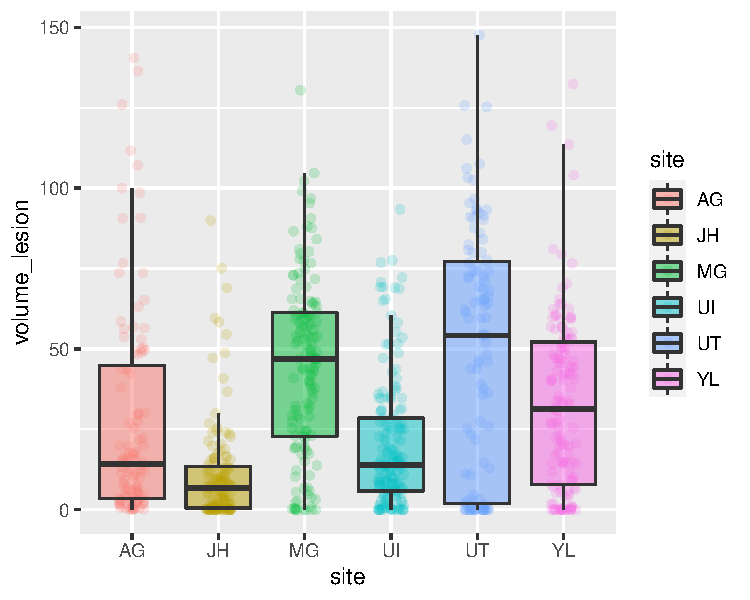
\includegraphics{paper_files/figure-latex/plot_lesion_early-1} \end{center}

\begin{table}[ht]
\centering
\begin{tabular}{rllrrrrrr}
  \hline
 & site & variable & num & mean & sd & min & max & cv \\ 
  \hline
1 & AG & volume\_lesion & 104 & 27.45 & 33.14 & 0.00 & 140.39 & 1.21 \\ 
  2 & JH & volume\_lesion & 137 & 10.86 & 15.66 & 0.00 & 89.85 & 1.44 \\ 
  3 & MG & volume\_lesion & 138 & 44.21 & 27.68 & 0.00 & 130.40 & 0.63 \\ 
  4 & UI & volume\_lesion & 162 & 20.05 & 20.15 & 0.00 & 93.31 & 1.00 \\ 
  5 & UT & volume\_lesion & 103 & 47.58 & 39.10 & 0.00 & 147.51 & 0.82 \\ 
  6 & YL & volume\_lesion & 128 & 32.92 & 27.34 & 0.00 & 132.32 & 0.83 \\ 
   \hline
\end{tabular}
\end{table}
\begin{table}[ht]
\centering
\begin{tabular}{rlrrrrrr}
  \hline
 & variable & num & mean & sd & min & max & cv \\ 
  \hline
1 & volume\_lesion & 772 & 29.54 & 30.03 & 0.00 & 147.51 & 1.02 \\ 
   \hline
\end{tabular}
\end{table}

\hypertarget{lesion-fraction-at-the-early-timepoint}{%
\section{Lesion fraction at the early
timepoint}\label{lesion-fraction-at-the-early-timepoint}}

\begin{center}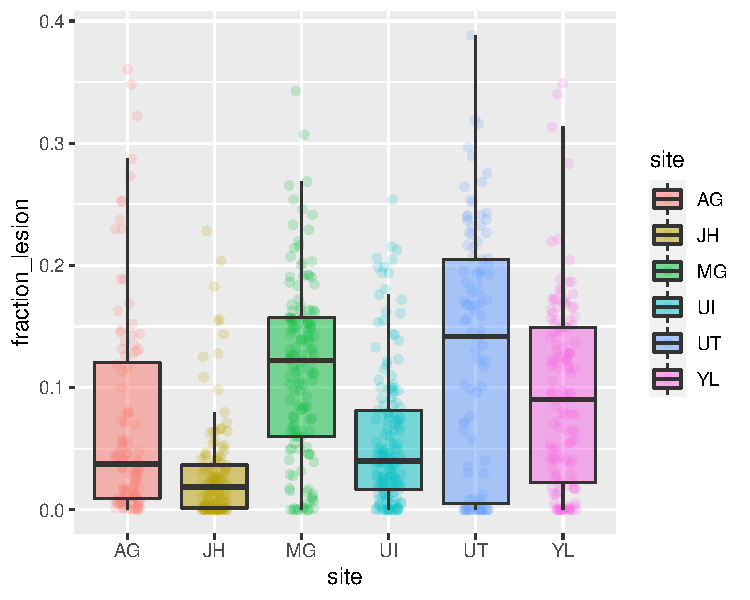
\includegraphics{paper_files/figure-latex/plot_fraction_lesion_early-1} \end{center}

\begin{table}[ht]
\centering
\begin{tabular}{rllrrrrrr}
  \hline
 & site & variable & num & mean & sd & min & max & cv \\ 
  \hline
1 & AG & fraction\_lesion & 104 & 0.07 & 0.09 & 0.00 & 0.36 & 1.19 \\ 
  2 & JH & fraction\_lesion & 137 & 0.03 & 0.04 & 0.00 & 0.23 & 1.42 \\ 
  3 & MG & fraction\_lesion & 138 & 0.11 & 0.07 & 0.00 & 0.34 & 0.63 \\ 
  4 & UI & fraction\_lesion & 162 & 0.06 & 0.06 & 0.00 & 0.25 & 0.99 \\ 
  5 & UT & fraction\_lesion & 103 & 0.13 & 0.10 & 0.00 & 0.39 & 0.81 \\ 
  6 & YL & fraction\_lesion & 128 & 0.09 & 0.08 & 0.00 & 0.35 & 0.82 \\ 
   \hline
\end{tabular}
\end{table}
\begin{table}[ht]
\centering
\begin{tabular}{rlrrrrrr}
  \hline
 & variable & num & mean & sd & min & max & cv \\ 
  \hline
1 & fraction\_lesion & 772 & 0.08 & 0.08 & 0.00 & 0.39 & 1.00 \\ 
   \hline
\end{tabular}
\end{table}

\hypertarget{csf-volume}{%
\section{CSF volume}\label{csf-volume}}

\begin{center}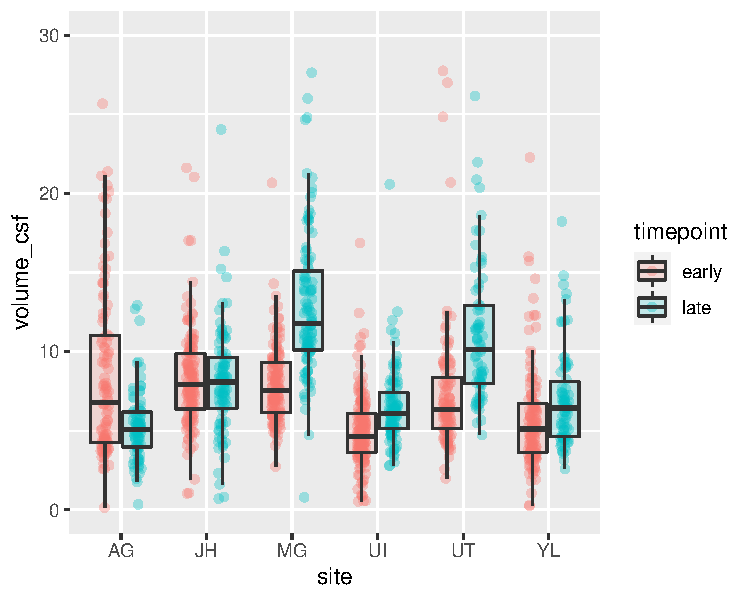
\includegraphics{paper_files/figure-latex/plot_csf_both-1} \end{center}

\begin{table}[ht]
\centering
\begin{tabular}{rlllrrrrrr}
  \hline
 & site & timepoint & variable & num & mean & sd & min & max & cv \\ 
  \hline
1 & AG & early & volume\_csf & 104 & 8.45 & 5.30 & 0.15 & 25.66 & 0.63 \\ 
  2 & AG & late & volume\_csf &  84 & 5.28 & 2.24 & 0.34 & 12.92 & 0.42 \\ 
  3 & JH & early & volume\_csf & 137 & 8.29 & 3.10 & 1.03 & 21.61 & 0.37 \\ 
  4 & JH & late & volume\_csf &  89 & 8.38 & 4.18 & 0.70 & 30.93 & 0.50 \\ 
  5 & MG & early & volume\_csf & 138 & 7.90 & 2.37 & 2.74 & 20.67 & 0.30 \\ 
  6 & MG & late & volume\_csf & 106 & 12.86 & 4.53 & 0.79 & 27.62 & 0.35 \\ 
  7 & UI & early & volume\_csf & 162 & 4.98 & 2.28 & 0.53 & 16.86 & 0.46 \\ 
  8 & UI & late & volume\_csf &  97 & 6.50 & 2.45 & 2.78 & 20.57 & 0.38 \\ 
  9 & UT & early & volume\_csf & 103 & 7.65 & 4.92 & 1.98 & 32.85 & 0.64 \\ 
  10 & UT & late & volume\_csf &  73 & 12.22 & 6.69 & 4.74 & 37.73 & 0.55 \\ 
  11 & YL & early & volume\_csf & 128 & 6.15 & 5.86 & 0.25 & 61.05 & 0.95 \\ 
  12 & YL & late & volume\_csf &  75 & 7.92 & 8.76 & 2.59 & 78.15 & 1.11 \\ 
   \hline
\end{tabular}
\end{table}
\begin{table}[ht]
\centering
\begin{tabular}{rllrrrrrr}
  \hline
 & timepoint & variable & num & mean & sd & min & max & cv \\ 
  \hline
1 & early & volume\_csf & 772 & 7.11 & 4.26 & 0.15 & 61.05 & 0.60 \\ 
  2 & late & volume\_csf & 524 & 8.91 & 5.83 & 0.34 & 78.15 & 0.65 \\ 
   \hline
\end{tabular}
\end{table}

\hypertarget{csf-fraction}{%
\section{CSF fraction}\label{csf-fraction}}

\begin{center}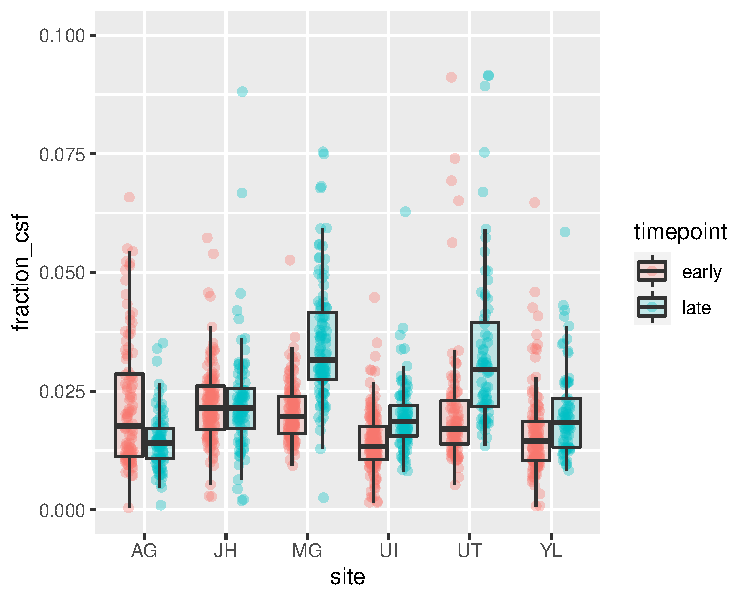
\includegraphics{paper_files/figure-latex/plot_fraction_csf_both-1} \end{center}

\begin{table}[ht]
\centering
\begin{tabular}{rlllrrrrrr}
  \hline
 & site & timepoint & variable & num & mean & sd & min & max & cv \\ 
  \hline
1 & AG & early & fraction\_csf & 104 & 0.02 & 0.01 & 0.00 & 0.07 & 0.61 \\ 
  2 & AG & late & fraction\_csf &  84 & 0.01 & 0.01 & 0.00 & 0.04 & 0.42 \\ 
  3 & JH & early & fraction\_csf & 137 & 0.02 & 0.01 & 0.00 & 0.06 & 0.37 \\ 
  4 & JH & late & fraction\_csf &  89 & 0.02 & 0.01 & 0.00 & 0.09 & 0.51 \\ 
  5 & MG & early & fraction\_csf & 138 & 0.02 & 0.01 & 0.01 & 0.05 & 0.29 \\ 
  6 & MG & late & fraction\_csf & 106 & 0.04 & 0.01 & 0.00 & 0.08 & 0.36 \\ 
  7 & UI & early & fraction\_csf & 162 & 0.01 & 0.01 & 0.00 & 0.04 & 0.44 \\ 
  8 & UI & late & fraction\_csf &  97 & 0.02 & 0.01 & 0.01 & 0.06 & 0.38 \\ 
  9 & UT & early & fraction\_csf & 103 & 0.02 & 0.01 & 0.01 & 0.09 & 0.64 \\ 
  10 & UT & late & fraction\_csf &  73 & 0.03 & 0.02 & 0.01 & 0.10 & 0.56 \\ 
  11 & YL & early & fraction\_csf & 128 & 0.02 & 0.02 & 0.00 & 0.16 & 0.88 \\ 
  12 & YL & late & fraction\_csf &  75 & 0.02 & 0.02 & 0.01 & 0.20 & 1.00 \\ 
   \hline
\end{tabular}
\end{table}
\begin{table}[ht]
\centering
\begin{tabular}{rllrrrrrr}
  \hline
 & timepoint & variable & num & mean & sd & min & max & cv \\ 
  \hline
1 & early & fraction\_csf & 772 & 0.02 & 0.01 & 0.00 & 0.16 & 0.57 \\ 
  2 & late & fraction\_csf & 524 & 0.02 & 0.02 & 0.00 & 0.20 & 0.64 \\ 
   \hline
\end{tabular}
\end{table}

\hypertarget{midline-shift}{%
\section{Midline shift}\label{midline-shift}}

\begin{center}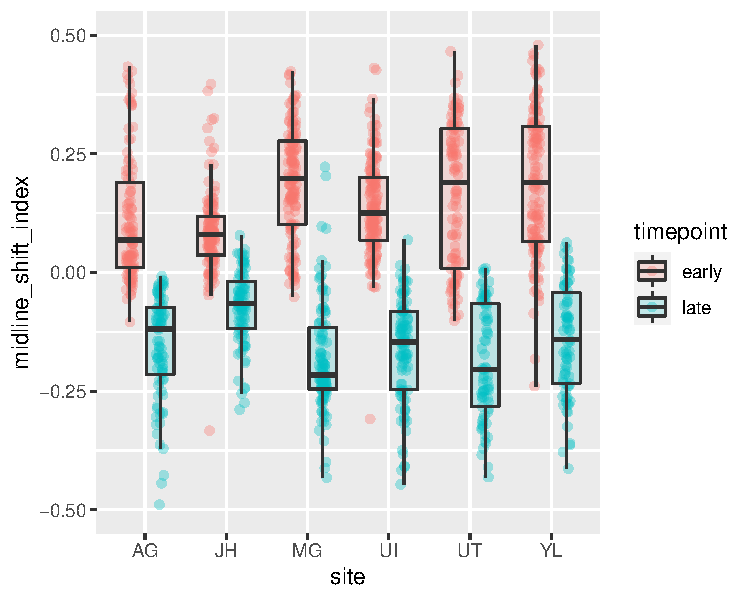
\includegraphics{paper_files/figure-latex/plot_shift_both-1} \end{center}

\begin{table}[ht]
\centering
\begin{tabular}{rlllrrrrrr}
  \hline
 & site & timepoint & variable & num & mean & sd & min & max & cv \\ 
  \hline
1 & AG & early & midline\_shift\_index & 104 & 0.11 & 0.13 & -0.10 & 0.43 & 1.21 \\ 
  2 & AG & late & midline\_shift\_index &  84 & -0.16 & 0.11 & -0.49 & -0.01 & -0.71 \\ 
  3 & JH & early & midline\_shift\_index & 137 & 0.09 & 0.09 & -0.33 & 0.40 & 1.01 \\ 
  4 & JH & late & midline\_shift\_index &  89 & -0.07 & 0.08 & -0.29 & 0.08 & -1.07 \\ 
  5 & MG & early & midline\_shift\_index & 138 & 0.19 & 0.12 & -0.05 & 0.42 & 0.61 \\ 
  6 & MG & late & midline\_shift\_index & 106 & -0.18 & 0.11 & -0.43 & 0.22 & -0.63 \\ 
  7 & UI & early & midline\_shift\_index & 162 & 0.14 & 0.11 & -0.31 & 0.68 & 0.80 \\ 
  8 & UI & late & midline\_shift\_index &  97 & -0.16 & 0.11 & -0.45 & 0.07 & -0.67 \\ 
  9 & UT & early & midline\_shift\_index & 103 & 0.17 & 0.16 & -0.10 & 0.50 & 0.94 \\ 
  10 & UT & late & midline\_shift\_index &  73 & -0.19 & 0.12 & -0.43 & 0.01 & -0.65 \\ 
  11 & YL & early & midline\_shift\_index & 128 & 0.19 & 0.15 & -0.24 & 0.48 & 0.80 \\ 
  12 & YL & late & midline\_shift\_index &  75 & -0.14 & 0.12 & -0.41 & 0.06 & -0.82 \\ 
   \hline
\end{tabular}
\end{table}
\begin{table}[ht]
\centering
\begin{tabular}{rllrrrrrr}
  \hline
 & timepoint & variable & num & mean & sd & min & max & cv \\ 
  \hline
1 & early & midline\_shift\_index & 772 & 0.15 & 0.13 & -0.33 & 0.68 & 0.89 \\ 
  2 & late & midline\_shift\_index & 524 & -0.15 & 0.11 & -0.49 & 0.22 & -0.76 \\ 
   \hline
\end{tabular}
\end{table}

\hypertarget{per-hemisphere-non-infarcted-tissue-fraction-at-the-early-timepoint}{%
\section{Per-hemisphere non-infarcted tissue fraction at the early
timepoint}\label{per-hemisphere-non-infarcted-tissue-fraction-at-the-early-timepoint}}

\begin{center}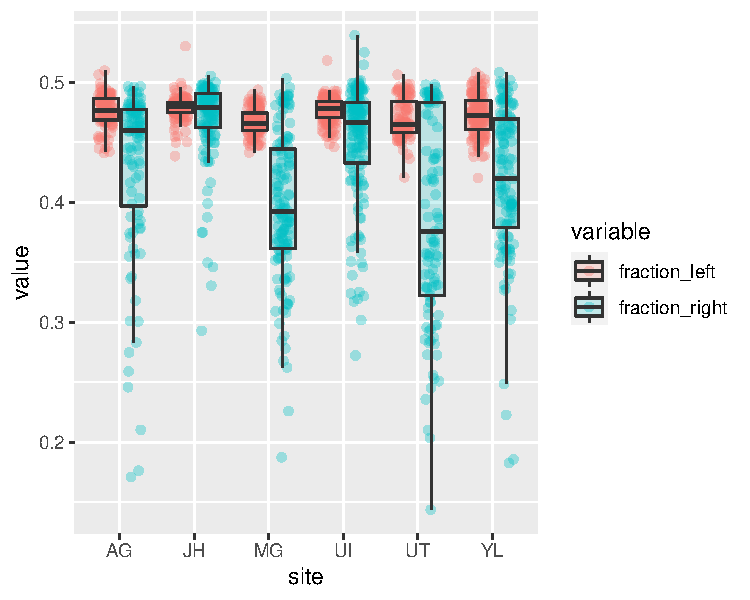
\includegraphics{paper_files/figure-latex/plot_hemi_early-1} \end{center}

\begin{table}[ht]
\centering
\begin{tabular}{rllrrrrrr}
  \hline
 & site & variable & num & mean & sd & min & max & cv \\ 
  \hline
1 & AG & fraction\_left & 104 & 0.48 & 0.01 & 0.44 & 0.51 & 0.03 \\ 
  2 & AG & fraction\_right & 104 & 0.43 & 0.07 & 0.17 & 0.50 & 0.17 \\ 
  3 & JH & fraction\_left & 137 & 0.48 & 0.01 & 0.44 & 0.53 & 0.02 \\ 
  4 & JH & fraction\_right & 137 & 0.47 & 0.03 & 0.29 & 0.51 & 0.07 \\ 
  5 & MG & fraction\_left & 138 & 0.47 & 0.01 & 0.44 & 0.49 & 0.02 \\ 
  6 & MG & fraction\_right & 138 & 0.40 & 0.06 & 0.19 & 0.50 & 0.15 \\ 
  7 & UI & fraction\_left & 162 & 0.48 & 0.01 & 0.45 & 0.52 & 0.02 \\ 
  8 & UI & fraction\_right & 162 & 0.45 & 0.05 & 0.27 & 0.54 & 0.11 \\ 
  9 & UT & fraction\_left & 103 & 0.47 & 0.02 & 0.42 & 0.51 & 0.03 \\ 
  10 & UT & fraction\_right & 103 & 0.38 & 0.09 & 0.14 & 0.50 & 0.22 \\ 
  11 & YL & fraction\_left & 128 & 0.47 & 0.02 & 0.42 & 0.51 & 0.04 \\ 
  12 & YL & fraction\_right & 128 & 0.42 & 0.06 & 0.18 & 0.51 & 0.15 \\ 
   \hline
\end{tabular}
\end{table}
\begin{table}[ht]
\centering
\begin{tabular}{rlrrrrrr}
  \hline
 & variable & num & mean & sd & min & max & cv \\ 
  \hline
1 & fraction\_left & 772 & 0.47 & 0.01 & 0.42 & 0.53 & 0.03 \\ 
  2 & fraction\_right & 772 & 0.43 & 0.07 & 0.14 & 0.54 & 0.16 \\ 
   \hline
\end{tabular}
\end{table}

\hypertarget{per-hemisphere-non-infarcted-tissue-fraction-at-the-late-timepoint}{%
\section{Per-hemisphere non-infarcted tissue fraction at the late
timepoint}\label{per-hemisphere-non-infarcted-tissue-fraction-at-the-late-timepoint}}

\begin{center}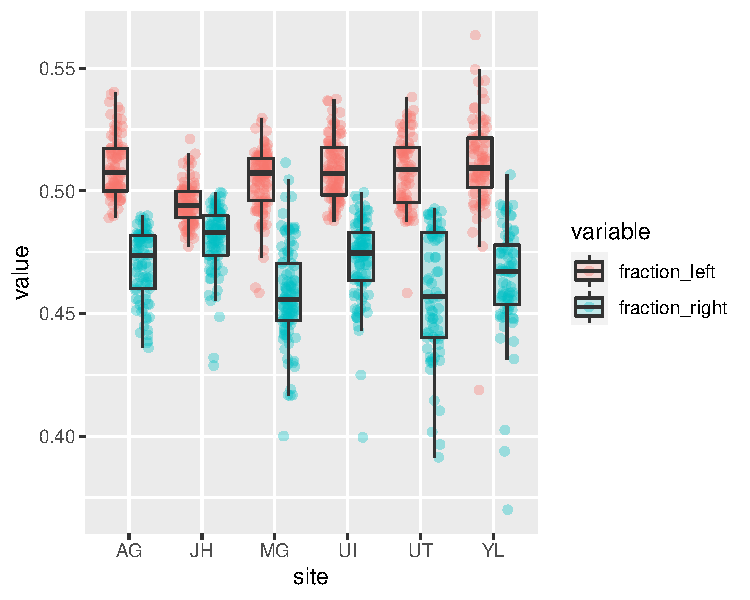
\includegraphics{paper_files/figure-latex/plot_hemi_late-1} \end{center}

\begin{table}[ht]
\centering
\begin{tabular}{rllrrrrrr}
  \hline
 & site & variable & num & mean & sd & min & max & cv \\ 
  \hline
1 & AG & fraction\_left &  84 & 0.51 & 0.01 & 0.49 & 0.54 & 0.02 \\ 
  2 & AG & fraction\_right &  84 & 0.47 & 0.01 & 0.44 & 0.49 & 0.03 \\ 
  3 & JH & fraction\_left &  89 & 0.49 & 0.01 & 0.48 & 0.52 & 0.02 \\ 
  4 & JH & fraction\_right &  89 & 0.48 & 0.01 & 0.43 & 0.50 & 0.03 \\ 
  5 & MG & fraction\_left & 106 & 0.50 & 0.01 & 0.46 & 0.53 & 0.02 \\ 
  6 & MG & fraction\_right & 106 & 0.46 & 0.02 & 0.40 & 0.51 & 0.04 \\ 
  7 & UI & fraction\_left &  97 & 0.51 & 0.01 & 0.49 & 0.54 & 0.02 \\ 
  8 & UI & fraction\_right &  97 & 0.47 & 0.02 & 0.40 & 0.50 & 0.03 \\ 
  9 & UT & fraction\_left &  73 & 0.51 & 0.02 & 0.46 & 0.54 & 0.03 \\ 
  10 & UT & fraction\_right &  73 & 0.46 & 0.03 & 0.39 & 0.49 & 0.06 \\ 
  11 & YL & fraction\_left &  75 & 0.51 & 0.02 & 0.42 & 0.56 & 0.04 \\ 
  12 & YL & fraction\_right &  75 & 0.46 & 0.02 & 0.37 & 0.51 & 0.05 \\ 
   \hline
\end{tabular}
\end{table}
\begin{table}[ht]
\centering
\begin{tabular}{rlrrrrrr}
  \hline
 & variable & num & mean & sd & min & max & cv \\ 
  \hline
1 & fraction\_left & 524 & 0.51 & 0.01 & 0.42 & 0.56 & 0.03 \\ 
  2 & fraction\_right & 524 & 0.47 & 0.02 & 0.37 & 0.51 & 0.04 \\ 
   \hline
\end{tabular}
\end{table}

\hypertarget{lesion-volume-vs-midline-shift-in-the-early-timepoint}{%
\section{Lesion volume vs midline shift in the early
timepoint}\label{lesion-volume-vs-midline-shift-in-the-early-timepoint}}

\begin{center}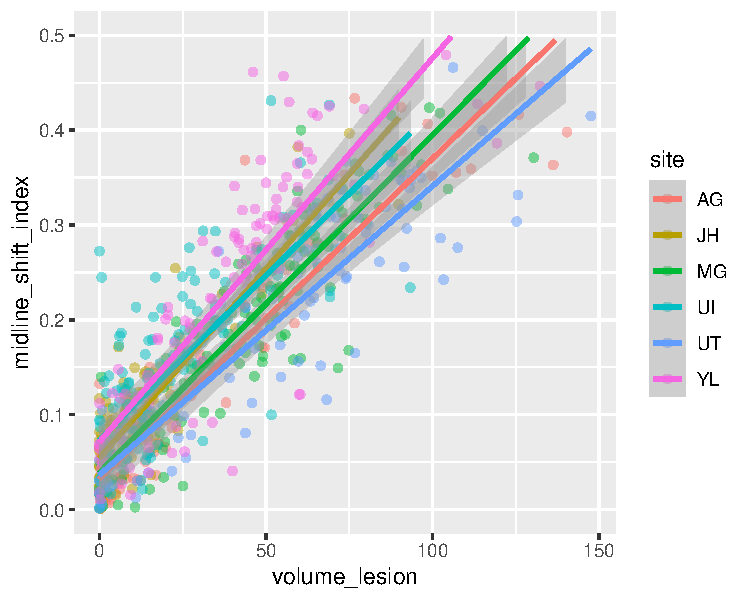
\includegraphics{paper_files/figure-latex/plot_lesion_shift-1} \end{center}

\hypertarget{early-timepoint-lesion-fraction-vs-late-timepoint-midline-shift}{%
\section{Early timepoint lesion fraction vs late timepoint midline
shift}\label{early-timepoint-lesion-fraction-vs-late-timepoint-midline-shift}}

\begin{center}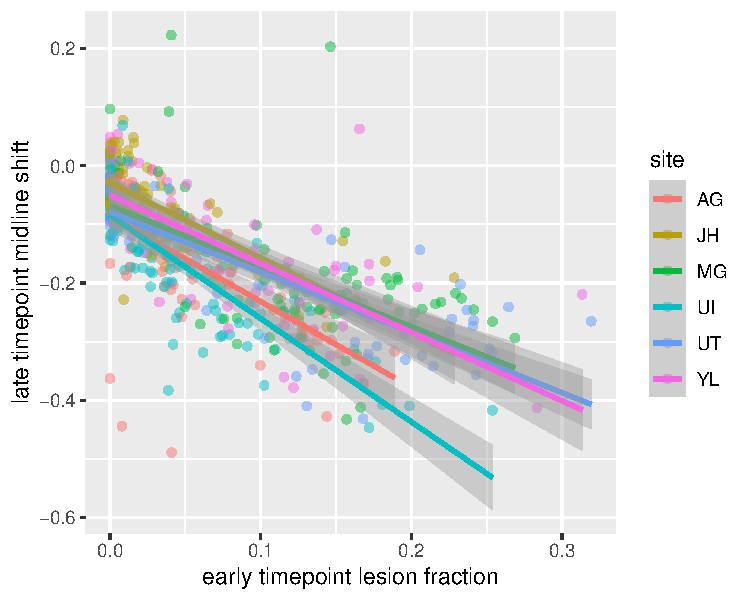
\includegraphics{paper_files/figure-latex/plot_lesion_shift_time-1} \end{center}

\end{document}
